% (5-20)
% 8 páginas

\chapter{Prova de Conceito: Estudo sobre Algoritmos de Agrupamento} \label{cap:estudo}

% Neste artigo será feita uma avaliação de quatro 

\begin{section}{Introdução}

No capítulo anterior foi mostrado que pelo menos três modelos geram redes organizadas em módulos que se assemelham a redes de software. Neste capítulo, o modelo BCR+ é usado em dois estudos experimentais realizados com o propósito de entender e comparar algoritmos de agrupamento que são estudados no contexto de recuperação de arquitetura de software. Os estudos são uma prova de conceito: eles demonstram a viabilidade do uso do modelo na avaliação de ferramentas de engenharia reversa.
%os algoritmos de agrupamento apresentados na Seção \ref{sec:algoritmos}.

Primeiramente, é feita uma breve introdução ao tema de algoritmos de agrupamento no contexto de recuperação de arquitetura. A seguir, são delineados os dois estudos sobre algoritmos de agrupamento. Por fim, são apresentados os resultados e as conclusões dos estudos.

\end{section}

\begin{section}{Agrupamento de Software}
	
Agrupamento é o processo de organizar entidades em módulos (ou grupos) de maneira que as entidades de um mesmo módulo sejam similares entre si segundo algum critério. (O termo agrupamento designa também o resultado do processo, que é a atribuição de entidades a módulos.) Um exemplo clássico é o agrupamento de pontos em um plano (entidades) de acordo com o critério da distância, como mostra a Figura \ref{fig:agrupamento}. O processo de agrupamento pode ser automatizado por meio de algoritmos, os quais têm sido objeto de estudo de áreas diversas como inteligência artificial, mineração de dados, análise de redes sociais, entre outras.

\begin{figure}[htbp]
	\centering
		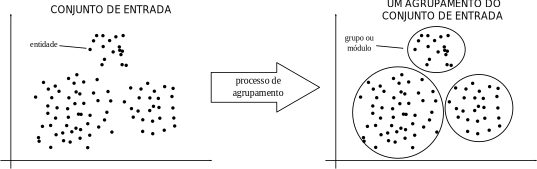
\includegraphics[scale=1]{figuras/agrupamento}
	\caption{O agrupamento de um conjunto de pontos no plano.}
	\label{fig:agrupamento}
\end{figure}

Algoritmos de agrupamento têm sido usados no contexto da engenharia de software para apoiar a atividade de recuperação de arquitetura, e nesse caso são chamados de \emph{algoritmos de agrupamento de software}. No início da atividade de recuperação de arquitetura, um algoritmo de agrupamento é aplicado a um sistema existente --- descrito, por exemplo, como uma rede de dependências entre classes, no qual as classes representam as entidades a serem agrupadas. O agrupamento encontrado serve como ponto de partida para a identificação manual dos módulos da arquitetura do sistema e das entidades que compõem cada módulo. 
% Uma das representações de sistemas empregadas nesse contexto é a rede de dependências entre entidades de código-fonte, já descrita em seções anteriores.

O conjunto de módulos de uma arquitetura e entidades associadas constituem um agrupamento, denominado agrupamento de referência. O objetivo de algoritmos de agrupamento de software, neste contexto, é encontrar agrupamentos similares aos agrupamentos de referência dos sistemas analisados \cite{Koschke2000}.

O custo de um experimento para avaliar algoritmos de agrupamento de software é elevado, uma vez que é necessário obter um agrupamento de referência para cada sistema analisado. Em uma avaliação feita por Girard e Koschke, quatro engenheiros de software levaram de 20 a 35 horas para obter agrupamentos de referência para programas na linguagem C com aproximadamente 30 mil linhas de código e apenas 40 entidades (tipos abstratos de dados) cada um \cite{Girard2000}. O alto custo de experimentos com algoritmos de agrupamento faz desse tipo de estudo um bom candidato à técnica de avaliação através de redes de software sintéticas.

%%%%%%%% TODO: Por que é interessante, nesta pesquisa, estudar rec. de arq? pq é difícil encontrar arqs. disponíveis, e é custoso gerá-las. Agrupamento de referência é difícil encontrar para vários sistemas e sistemas diversos.

\end{section}

\begin{section}{Delineamento Experimental}
	
	A fim de comparar algoritmos de agrupamento e de entender os fatores que influenciam o seu desempenho, dois experimentos foram realizados. O primeiro experimento teve como propósito comparar o desempenho dos algoritmos de agrupamento sob o critério da semelhança dos agrupamentos encontrados pelos algoritmos com agrupamentos de referência. O segundo experimento teve como propósito entender como o desempenho dos algoritmos é afetado por parâmetros que descrevem cada rede.
	
	Os métodos e materiais dos dois experimentos são semelhantes e, por isso, são discutidos conjuntamente nesta seção. Os experimentos consistem nas seguintes etapas: 
\begin{enumerate}
	\item gerar redes usando diversas combinações de valores para os parâmetros do modelo BCR+;
	\item aplicar algoritmos de agrupamento a cada uma das redes;
	\item aferir o desempenho dos algoritmos de agrupamento em cada rede, isto é, medir a similaridade entre os agrupamentos encontrados pelos algoritmos e os agrupamentos de referência. O agrupamento de referência de uma rede, neste caso, é determinado pelos próprios módulos gerados pelo modelo BCR+;
	\item interpretar os resultados.
\end{enumerate}

	A escolha do modelo BCR+ se deve à familiaridade do autor com as propriedades do modelo. Os estudos tiveram como ponto de partida as 9.500 configurações de parâmetros descritas no experimento de avaliação de software-realismo, na Seção \ref{sec:parametros}. Com a finalidade de mitigar os efeitos aleatórios na geração de redes, para cada configuração foram geradas três redes, totalizando 28,5 mil redes.

	Para este estudo foram escolhidos algoritmos de agrupamento que possuem implementação disponível na Web e que já foram estudados por mais de um autor em pesquisas sobre recuperação de arquitetura. De acordo com esse critério, foram escolhidos os algoritmos ACDC, Bunch e algoritmos hierárquicos aglomerativos (ligação simples, SL, e ligação completa, CL), descritos no Apêndice \ref{cap:agrupamento}. Para cada um dos algoritmos aglomerativos, foram estudadas duas alturas de corte\footnote{Em um algoritmo aglomerativo, a altura de corte influencia o número de módulos identificados: quanto maior a altura de corte, menor o número de módulos (e, consequentemente, maior o tamanho médio dos módulos).}, $0,75$ e $0,90$. No total são 4 configurações de algoritmos aglomerativos, que serão referenciadas como SL75, SL90, CL75 e CL90. Para os algoritmos Bunch e ACDC foram escolhidas as configurações padrão das implementações dos autores dos algoritmos. As 6 configurações escolhidas para este estudo são idênticas àquelas estudadas por Wu, Hassan e Holt \cite{Wu2005} (maiores informações no Capítulo \ref{cap:trabrel}).
	
	Para medir a similaridade entre agrupamentos, foi escolhida a métrica MoJoSim \cite{Tzerpos1999,Bittencourt2009}, que tem sido usada em estudos sobre agrupamento de software para recuperação de arquitetura. Em poucas palavras, a métrica MoJoSim mede, em uma escala contínua de 0 a 1, o esforço necessário para se transformar no agrupamento de referência um agrupamento dado. O valor 1 indica que os dois agrupamentos comparados são idênticos (e o esforço é, portanto, nulo). 
	
	Na métrica MoJoSim, considera-se que o esforço envolvido em unir dois módulos é pequeno se comparado ao esforço de dividir um módulo em dois. A justificativa é que, para dividir um módulo em dois, é preciso analisar cada entidade e determinar para qual módulo ela deve ser movida.

% , explicada no Apêndice \ref{cap:mojosim}

	A partir dos dados coletados foram realizadas análises gráficas e testes de hipóteses. Uma análise preliminar revelou que os dados, em geral, não obedecem a uma distribuição normal, e por isso foram usados testes de hipótese não-paramétricos --- testes que não assumem os dados seguem uma distribuição de probabilidade determinada. A variável dependente é, em ambos os experimentos, o desempenho de um determinado algoritmo em uma determinada rede, medido pela métrica MoJoSim. As variáveis independentes são os parâmetros do modelo BCR+ e a escolha do algoritmo de agrupamento.
	
	% O teste de Wilcoxon é um teste não paramétrico cuja hipótese nula é a de que, escolhidos dois elementos, um de cada amostra, a probabilidade de que o primeiro seja maior do que o segundo é aproximadamente igual a 50\%. A hipótese alternativa é que os valores de uma amostra tendem a ser maiores do que os valores da outra. Ao contrário do teste de t-Student para comparação de médias de populações, o teste de Wilcoxon não assume que os dados seguem uma distribuição normal.
	

	% A base dos experimentos são testes de hipótese, nos quais se verificam hipóteses do tipo ``o algoritmo ACDC possui maior desempenho do que o algoritmo CL90''. Verificou-se, no entanto, que a distribuição dos valores de MoJoSim não é normal, o que descarta o teste de t-Student para a comparação de duas amostras. Por essa razão foram utilizados testes não-paramétricos, como o teste de Mann-Whitney, cuja validade não depende da suposição de que a distribuição é normal.
\end{section}

\begin{section}{Experimento 1: Comparação entre Algoritmos}

O primeiro experimento teve como objetivo comparar o desempenho dos algoritmos de agrupamento com relação à similaridade entre agrupamentos encontrados pelos algoritmos e os agrupamentos de referência correspondentes.

Cada algoritmo foi aplicado a cada uma das redes sintéticas, resultando em agrupamentos cujo desempenho foi medido pela métrica MoJoSim. Apenas redes software-realistas (valor $S \ge 0,88$), totalizando quase 6 mil redes, foram usadas neste estudo, uma vez que o objetivo é comparar o desempenho de algoritmos quando aplicadas a redes de software.

% falar que quartis são métricas robustas?
A Figura \ref{fig:box-mojo-por-alg} mostra um \emph{boxplot} dos valores de MoJoSim alcançados por cada algoritmo. No \emph{boxplot}, o retângulo vai do quartil inferior (Q1) até o quartil superior (Q3), com a mediana desenhada como uma linha horizontal dentro do retângulo. Q1 representa o valor que é maior do que 25\% dos valores e Q3 representa o valor que é maior do que 75\% dos valores. Acima e abaixo do retângulo estão linhas horizontais que indicam o valor mínimo e o valor máximo do conjunto de dados. % As linhas são limitadas por Q1 - (1.5 * IQR) e Q3 + (1.5 * IQR)...

\begin{figure}[htbp]
	\centering
		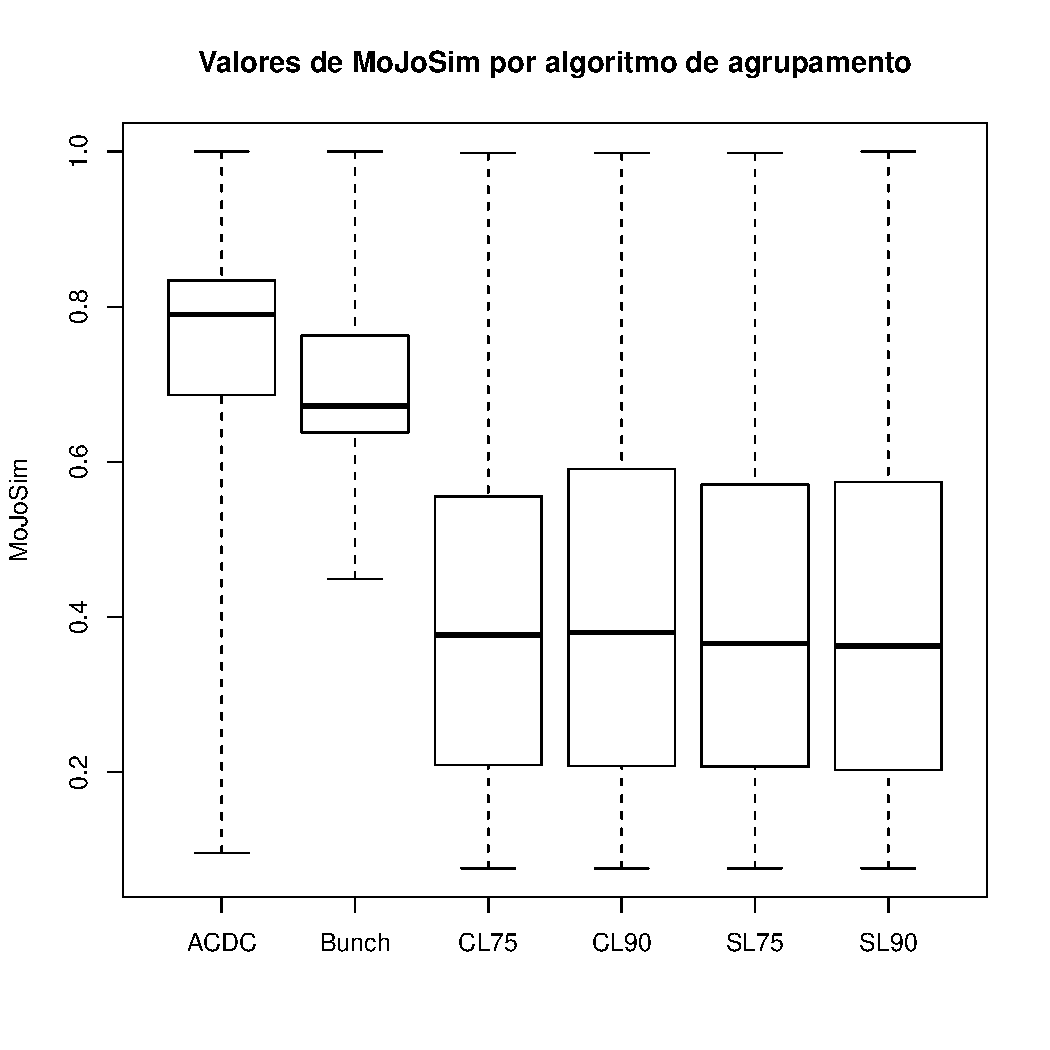
\includegraphics[scale=0.5]{figuras/box-mojo-por-alg}
	\caption{Resumo estatístico dos valores de MoJoSim de cada algoritmo de agrupamento.}
	\label{fig:box-mojo-por-alg}
\end{figure}

Comparando pelo gráfico os MoJoSims medianos de cada algoritmo, nota-se que o algoritmo ACDC apresenta o melhor desempenho, seguido do Bunch. A seguir vêm os algoritmos aglomerativos, com pequenas diferenças entre si. A fim de verificar se as diferenças observadas são estatisticamente significativas, foi aplicado o teste de Wilcoxon pareado para as medianas de cada par de algoritmos, com nível de significância igual a 5\%. (Para mitigar o efeito que a aplicação de múltiplos testes exerce sobre a significância estatística, foi usada a correção de Bonferroni, que consiste em dividir o nível de significância pelo número de testes realizados, reduzindo a probabilidade de se obter falsos positivos.) Os testes confirmaram as conclusões feitas a partir do gráfico, mas não foi encontrada nenhuma evidência de que algum algoritmo aglomerativo se destaque sobre os demais.


% Em uma análise complementar, foi selecionado de cada rede o algoritmo de maior desempenho e então contou-se a proporção de redes em que cada algoritmo foi o melhor, como mostra a Figura XXX. Essa análise confirma a superioridade dos algoritmos ACDC e Bunch no conjunto das redes estudadas. Mais do que isso, observa-se que os algoritmos aglomerativos dividem de forma quase igualitária o posto de melhor algoritmo nos casos que não são dominadas pelo ACDC ou pelo Bunch.

Outro aspecto a se observar é a dispersão dos valores. O algoritmo Bunch é o que apresenta a menor dispersão dentre os algoritmos analisados, com mais de 50\% dos valores de MoJoSim na faixa de $0,60$ a $0,80$, e menor MoJoSim igual a $0,45$. No caso do ACDC, 50\% dos valores de MoJoSim estão entre $0,65$ e $0,85$, porém o valor mínimo é $0,01$. Esta observação sugere que o algoritmo Bunch, embora apresente desempenho inferior ao ACDC na maioria dos casos, pode ser uma escolha interessante pelo fato de ter um desempenho mais previsível.

O resultado encontrado diverge das conclusões de Wu, Hassan e Holt \cite{Wu2005}. Eles concluíram que os algoritmos, ordenados do melhor desempenho para o pior, são CL90, CL75, Bunch, ACDC, SL75, SL90. As divergências provavelmente se explicam pelos critérios empregados para definir o agrupamento de referência. No estudo deles, o agrupamento de referência foi extraído da estrutura de diretórios do código-fonte dos sistemas estudados; neste estudo, o agrupamento de referência é definido \emph{a priori}, e as redes são geradas de forma a reduzir as dependências entre módulos.

Vale ressaltar que, apesar de uma amostra grande ter sido usada no estudo, as conclusões não são definitivas. O teste do valor S garante que todas as redes da amostra são software-realistas, mas não é possível afirmar que as redes software-realistas estejam bem representadas na amostra. Possivelmente o modelo BCR+ não é capaz de gerar certos tipos de redes software-realistas, o que potencialmente introduz um viés no experimento que pode beneficiar um algoritmo ou outro. Ainda assim, esta análise complementa estudos de caso realizados por outros autores \cite{Wu2005,Andritsos2005}, que são viesados pelo fato de analisarem uma amostra pequena de sistemas de software.

\end{section}

\begin{section}{Experimento 2: Estudo de Parâmetros}

O segundo experimento teve como objetivo estudar como o desempenho dos algoritmos é afetado pela variação de parâmetros do modelo. 

O experimento seguiu uma configuração fatorial completa: considerando que cada parâmetro do modelo BCR+ pode assumir os valores discretos determinados na Seção \ref{sec:parametros}, foram estudadas redes geradas a partir de todas as combinações de valores discretos para cada parâmetro do modelo. Tal configuração experimental permite estudar isoladamente o efeito de cada parâmetro sobre o desempenho de um algoritmo, algo que não é possível em estudos de caso.

Vale destacar que, neste caso, foram estudadas tanto redes software-realistas quanto redes não software-realistas, pois apenas desta forma é possível isolar cada parâmetro. Considere duas amostras das redes do estudo: a primeira composta de todas as redes com $\mu = 0,2$ e a segunda composta de todas as redes com $\mu = 0,4$. Exceto pelo valor de $\mu$, cada combinação de valores de parâmetros na primeira amostra está presente também na segunda amostra e vice-versa. Assim, qualquer diferença entre os MoJoSim médios das amostras pode ser atribuído exclusivamente à variação no valor de $\mu$ e a efeitos aleatórios. Tal conclusão não seria válida se apenas redes software-realistas fossem analisadas. Nesse caso, não haveria uma correspondência completa entre as redes das duas amostras, e essa diferença entre as amostras também afetaria o valor de MoJoSim. Não seria possível, portanto, isolar a contribuição do parâmetro $\mu$ no resultado.

% balanceado: cada tratamento tem o mesmo número de participantes (três)
% replicado: cada tratamento tem mais de um participante (três)

% O número de tratamentos aumenta muito com o aumento do número de
% níveis e de fatores, tornando praticamente impossível distribuí-los em blocos
% casualizados, devido à exigência de homogeneidade das parcelas dentro de
% cada bloco.

%casualização = sorteio

% uniformidade da amostra

% A primeira questão estudada foi a seguinte: os algoritmos apresentam melhor desempenho com redes software-realistas? Para responder a essa pergunta, as redes foram divididas em dois grupos (software-realistas e não software-realistas) e os valores de MoJoSim dos grupos foram comparados através do teste de Mann-Whitney (Wilcoxon não-pareado), com 5\% de significância. O teste forneceu evidências de que os algoritmos CL75, CL90, ACDC e Bunch apresentam melhor desempenho quando aplicados a redes software-realistas. O teste foi inconclusivo com relação aos algoritmos SL75 e SL90. As diferenças entre os dois grupos de redes são ilustradas no histograma da Figura XXX.

Um ponto que chamou a atenção foi a relação entre o desempenho dos algoritmos e o número de módulos do agrupamento de referência de cada rede. Nos algoritmos aglomerativos, um aumento no número de módulos provoca uma piora do desempenho; nos demais algoritmos, não há uma variação significativa. Este fenômeno pode ser observado no gráfico da Figura \ref{fig:mojosim-vs-modules} e foi confirmado através do teste de Wilcoxon pareado com 5\% de significância. Esse é um comportamento, portanto, que diferencia os algoritmos aglomerativos dos demais. 

\begin{figure}[htbp]
	\centering
		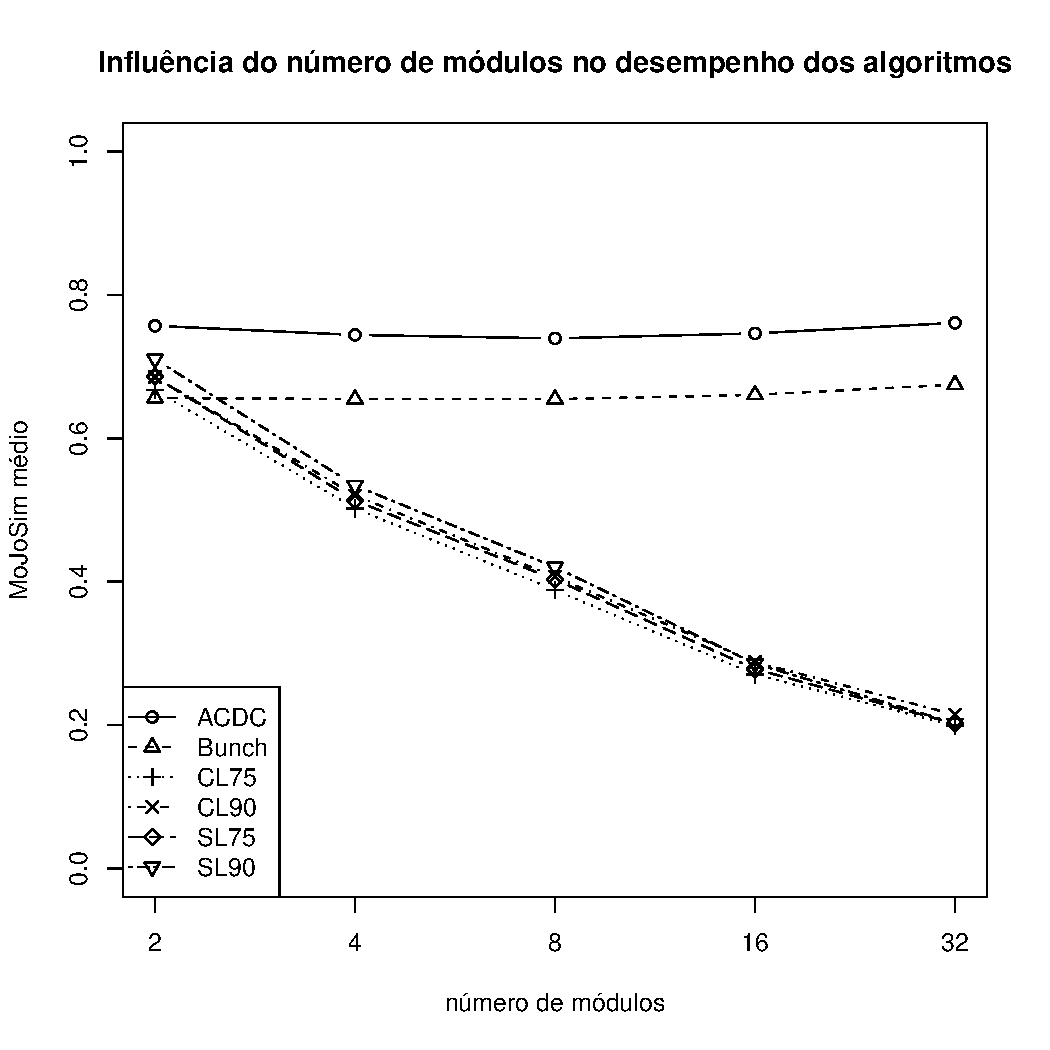
\includegraphics[scale=0.5]{figuras/mojosim-vs-modules}
	\caption{Influência do número de módulos do agrupamento de referência no desempenho de cada algoritmo de agrupamento.}
	\label{fig:mojosim-vs-modules}
\end{figure}

Uma possível explicação está na distribuição dos tamanhos dos módulos encontrados pelos algoritmos aglomerativos. Nestes, é comum serem encontrados módulos muito grandes, às vezes contendo mais da metade da rede \cite{Wu2005}. Quando o agrupamento de referência possui muitos módulos, os módulos grandes encontrado pelo algoritmo precisam ser divididos em diversos módulos menores, uma operação que é bastante penalizada na métrica MoJoSim.

% A Tabela XXX mostra o comportamento do desempenho dos algoritmos com o aumento dos valores de cada parâmetro. Em geral, observa-se que o desempenho piora quando os valores dos parâmetros aumentam.

\end{section}

\begin{section}{Conclusão}

Os estudos experimentais descritos neste capítulo mostraram que, quando aplicado a redes software-realistas, o algoritmo ACDC apresenta melhor desempenho que o algoritmo Bunch, enquanto os algoritmos aglomerativos possuem desempenho inferior. O desempenho dos algoritmos aglomerativos pode, em parte, ser explicado pela sua dificuldade de lidar com redes que possuem muitos módulos. Tal dificuldade foi comprovada em um experimento que isolou a influência do número de módulos no desempenho dos algoritmos. Apenas os algoritmos aglomerativos foram afetados pela variação no número de módulos.

\end{section}
